%%%% final_report.tex
%% Search Final Project
%% Ryder McMinn

\typeout{Search Final Project}

% Latex Template modified from IJCAI-19 template.

\documentclass{article}
\pdfpagewidth=8.5in
\pdfpageheight=11in
% The file ijcai19.sty is NOT the same than previous years'
\usepackage{ijcai19}

% Use the postscript times font!
\usepackage{times}
\usepackage{soul}
\usepackage{url}
\usepackage[hidelinks]{hyperref}
\usepackage[utf8]{inputenc}
\usepackage[small]{caption}
\usepackage{graphicx}
\usepackage{amsmath}
\usepackage{booktabs}
\urlstyle{same}

% the following package is optional:
%\usepackage{latexsym} 

\title{Search Final Project}

\author{
Ryder McMinn\\
\affiliations
Indiana University - Bloomington\\
\emails
rmcminn@iu.edu
}

\begin{document}

\maketitle

\begin{abstract}
	Code located here:\\ \url{https://github.com/mcminnra/search_final_project}
\end{abstract}

\section*{Introduction}

In this final project, we will attempt two tasks working off the Yelp dataset (\url{https://www.yelp.com/dataset}). In the first task, our goal is be able to predict the categories of a business using textual features. In the second task, I picked applying Youtube's Deep Recommendation approach \cite{youtubedeep} to the Yelp Dataset to be able to recommend businesses to users.

\section*{Task 1 - Multi-Label Classification for Yelp Business Categories}

In this task, our goal is to build a model that is able to predict the categories of a Yelp business. Our approach was to use the text in user reviews plus the business's title to be able to generate predictions of that business's Yelp categories (See Figure \ref{fig:yelp_categories}.)

\begin{figure}[h!]
	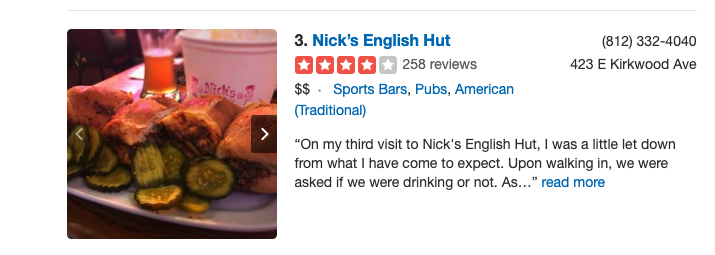
\includegraphics[width=\linewidth]{img/yelp_categories.png}
	\caption{Photo of a local business with it's associated categories.}
	\label{fig:yelp_categories}
\end{figure}

\subsection*{Data Preprocessing}

For task 1, we took a a couple of steps to preprocess the review text before we attempted learning. After some testing, we realized that including the business's title significantly improved performance without affecting preprocessing or training time in any meaningful way. Upon this combination of each review and it's associated business's title, we then removed all punctuation marks and stop words \cite{wiki:stopwords}; removing the punctuation marks allowed us to tokenize the text easier, and removing the stop words deleted words that provided little to no predictive value. This also had the result of speeding up training time, and reducing the training corpus. 

After these steps, we sought to normalize the text. Normalization allows us to reduce the overall corpus by either stemming \cite{wiki:stem} each word to a root spelling or to convert a word to it's associated lemma via lemmatization \cite{wiki:lemma}. This has the effect of reducing training time and increasing accuracy because it more concisely captures a words semantic meaning in all it's various forms, declensions, and conjugations. Looking at Table 1, we can see that stemming is the best approach for our review data. I suspect this has to do with the fact that you lose some semantic meaning with lemmatization. For example, 'great' becomes 'good' and 'awesome' becomes 'good', since 'good' is the lemma of both of these words. However, you lose the information that 'great' and 'awesome' provide. These offer different interpretations of 'good' that have some meaning in the context of a review or business. Losing this information means we lose some predictive value when training. With no word normalization, we then have to train on all the various forms of a word. In this case, we don't lose predictive value, instead, we don't have enough training data to be able to capture all the variations. For example, 'greater', 'greatly', and 'greatness' are all forms of 'great', and if we don't reduce them to just 'great', we need many more examples of each of these to be able to capture the information that 'great' provides. In essence, we may gain some accuracy when we have an immense amount of data, but when we have relatively few examples, it fails to learn each of them, which instead it can learn if we reduce all of them to just 'great'. 

%% Normalization Comparision
\begin{table}[h!]
	\begin{center}
		\caption{Normalization Comparison over 200,000 Reviews (\textbf{Best Results in Bold})}
		\label{tab:table1}
		\begin{tabular}{l||c|c|r} % <-- Alignments: 1st column left, 2nd middle and 3rd right, with vertical lines in between
			\textbf{} & \textbf{Stemming} & \textbf{Lemmatization} & \textbf{None}\\
			\hline
			Preprocessing (min.) & \textbf{21.06} & 25.16 & 27.58\\
			Training (min.) & \textbf{13.55} & 14.58 & 14.86\\
			Train Loss & .0048 & .0048 & \textbf{.0047}\\
			Validation Loss & \textbf{.0070} & .0071 & .0071\\
			Test Loss & \textbf{.0069} & .0070 & .0071\\
		\end{tabular}
	\end{center}
\end{table}

After normalization, we converted our reviews to a sequence of word ids and padded them with zeros, so they are all the same length. This will allow us to do convolutions over our text data (e.g. [14, 23, 2, 67, 0, 0, 0, 0])

\subsection*{Approach and Architecture}

Our approach to generating these categories was to use trained word embeddings and then apply a convolution layer over them (See Architecture below)

\mbox{}\\
\begin{verbatim}
Embedding Layer (length=50)
\end{verbatim}
$\downarrow$
\begin{verbatim}
1-D Convolution Layer
(filters=128,
 filter_size=5,
 activation='relu')
\end{verbatim}
$\downarrow$
\begin{verbatim}
Global Max Pooling Layer
\end{verbatim}
$\downarrow$
\begin{verbatim}
Dense Layer (neurons=1000)
\end{verbatim}
$\downarrow$
\begin{verbatim}
Softmax Output(1300 categories)
\end{verbatim}
\mbox{}\\

We trained out output layer using Binary Crossentropy loss in order to be able to learn multiple categories (Multi-Label) on output. From personal experience if each text example is short (like a review), and contains natural spoken speech patterns, the best approach is to simply use the above architecture of WordEmbeddings+CNN. I tried added an LSTM layer, but since more reviews were short and contained natural speech, the LSTM had trouble finding key dependencies to remember that would improve performance. The result was significantly increasing training time, while not improving performance. I, also, tried using a simple Multi-Layer Perception with TFIDF, but the feature size grew exponentially large, and made meaningful training impossible. Memory became a huge bottleneck and prohibited using large data sizes for training

\subsection*{Results}

Here you'll see my best model results. I ran out of time to do comparisons to previous iterations and techniques unfortunately. 



\subsection*{Final Results}

\section*{Task 2 - Deep Recommendation}

\subsection*{Data Preprocessing}

\subsection*{Approach and Architecture}

\subsection*{Results}

\subsection*{Final Results}

\medskip

\bibliographystyle{unsrt}
\bibliography{final_report}

\end{document}